\section{Quantum Circuits}

This section briefly reviews the gate model for circuit based quantum computing and discusses the similarities between between digital and quantum computers. The gate model is one of the most popular architectures for quantum computation at the moment. \textit{Intel \cite{intelqcomp} IBM \cite{ibmqweb}, Google \cite{googleqai}, Rigetti \cite{rigetti}} \textbf{REF!} are all using the gate model approach for quantum computing.

Both forms of computation follow the same structure, you start with bits (or qubits), operations are performed on the (qu)bits and then you measure the new values of the (qu)bits. We show an example in \autoref{fig:basicoperation}.

%%%% digital circuit
\begin{figure}[H] 
\centering
\begin{subfigure}[h]{0.4\textwidth}
\begin{align*}
\Qcircuit @C=0.5cm @R=0.7cm
{&\lstick{A} &\multigate{2}{Operation} & \\
&\lstick{B} &\ghost{Operation} & \\
&& &\qw &\lstick{Q} \\}
\end{align*}
\caption{Digital operation}
\label{fig:digitalcirc}
\end{subfigure}
~
%%%% Q circuit
\begin{subfigure}[H]{0.4\textwidth}
\begin{align*}
\Qcircuit @C=0.5cm @R=0.7cm
{&\lstick{A} &\multigate{2}{Operation} &\qw &\lstick{A} \\
&\lstick{B} &\ghost{Operation} &\qw &\lstick{B} \\
&\lstick{Q} &\ghost{Operation} &\qw &\lstick{Q} \\}
\end{align*}
\caption{Quantum operation}
\label{fig:quantumcirc}
\end{subfigure}
\caption{resource flow}
\label{fig:basicoperation}
\end{figure}

This  

\subsubsection{Digital logic}

Every digital computing operation can be built up from NAND logic gates \cite{sheffer1913set}. We call this a universal gate for computation.

\begin{figure}[h]
  \centering
  \begin{subfigure}[h]{0.4\textwidth}
  \centering
  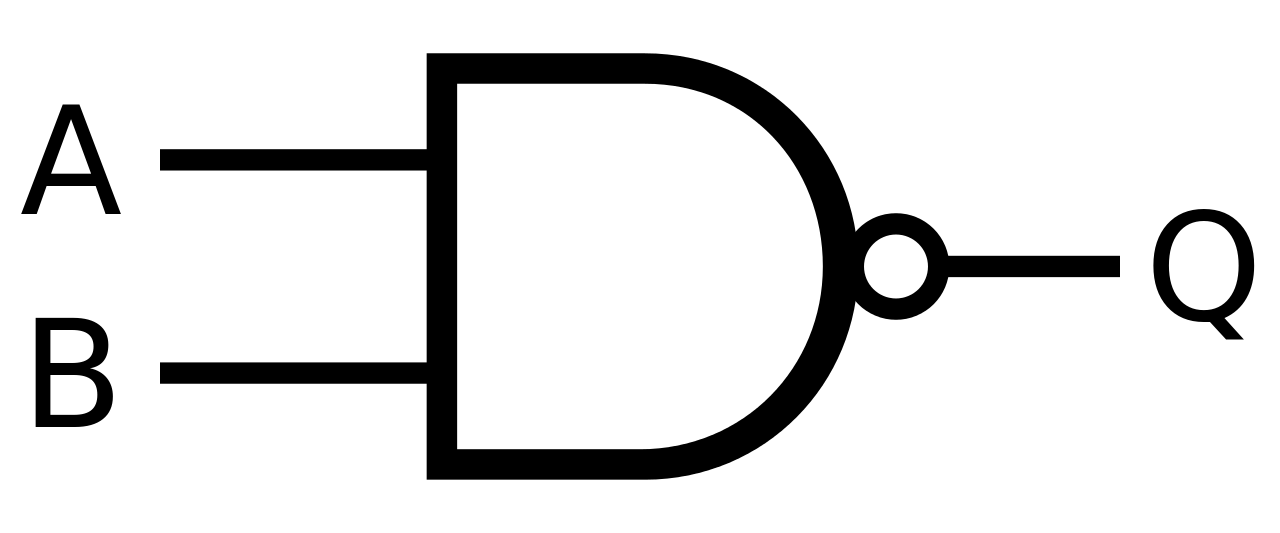
\includegraphics[width=0.7\textwidth]{NAND_ANSI_Labelled_svg.png}
  \caption{The NAND logic gate \cite{nandwiki}.}
  \label{fig:NAND}
\end{subfigure}
~
  \begin{subfigure}[h]{0.4\textwidth}
  \centering
  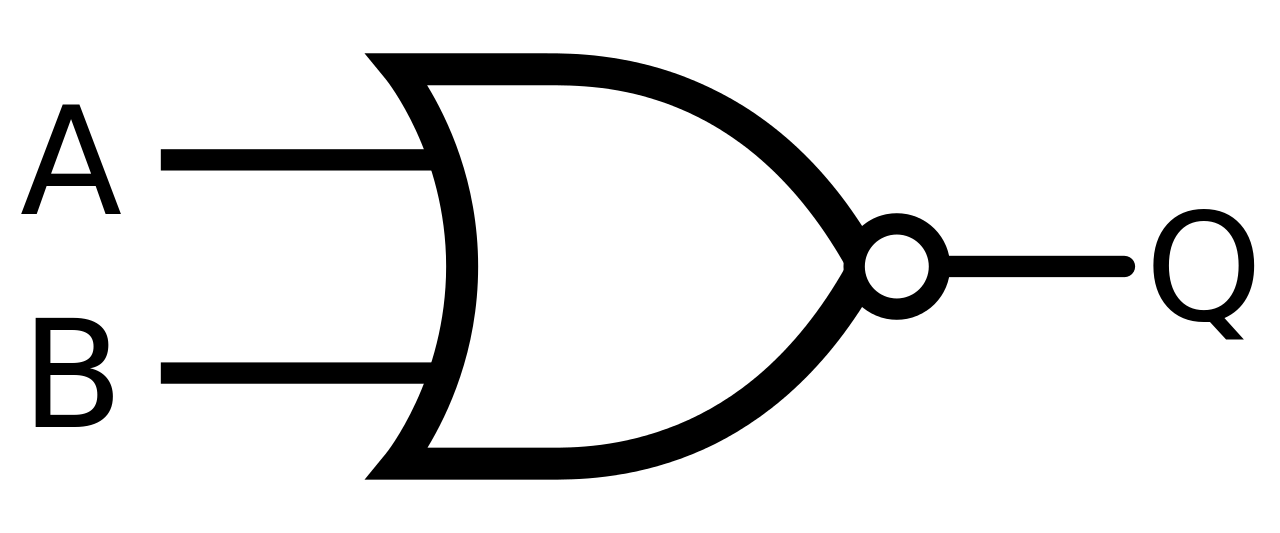
\includegraphics[width=0.7\textwidth]{NOR_ANSI_Labelled_svg.png}
  \caption{The NOR logic gate \cite{norwiki}.}
  \label{fig:NOR}
  \end{subfigure}
\end{figure}

reversible logic

%%%%%%%%% circuit 1 
\begin{figure}[h!]
\begin{align*}
\Qcircuit @C=0.5cm @R=0.7cm
{%1
&\lstick{S_1} &\gate{H} &\ctrl{1} &\qw \\
%0
&\lstick{S_0} &\ctrl{-1} &\targ &\qw \\}
\end{align*}
\caption{Schur transform for 2 qubits}
\label{cir:vanilla2}
\end{figure}

